\documentclass[e4_tp3_main.tex]{subfiles}
\begin{document}
\newgeometry{top=2.5cm, bottom=2.0cm, left=2.25cm, right=2.25cm}

\section{Inverter Trifásico}

\subsection{Generación PWM y Disparo}

\subsubsection{Overlapping}

Debido a los tiempos de encendido y apagado de los transistores, puede haber un tiempo durante el cual, al conmutar, estén ambos encendidos (de la misma rama del inverter). Una forma de minimizar este tiempo, es proporcionar un camino en Gate a través de un diodo para que el capacitor $C_{gd}$ del MOS se descargue más rápido. Se coloca una resistencia en paralelo para dar un camino a Gate en el encendido, como se muestra en la figura.

\begin{figure}[H]
\centering
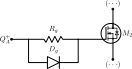
\includegraphics[width=0.6\linewidth]{Imagenes/overlap.png}
\caption{Inverter Trifásico - Minimización de Overlapping}
\end{figure}

\subsubsection{Generación de señales con $\mathbf{\mu}$P}

Para la generación de las señales de control, tendría una tabla principal (en este caso con 512 puntos), donde se compararía cada punto con el valor actual de la señal triangular generada en paralelo. Siendo 50Hz la frecuencia buscada de recorrido de la tabla, el período es de 20ms, por lo que debería realizarse una comparación cada:
\[
t_{COMP} = \frac{20ms}{512} = 39us \Longrightarrow f_{COMP} = \frac{1}{t_{COMP}} = 25.6KHz 
\]
Es decir que, por lo menos la frecuencia de clock debe ser de 25.6KHz para recorrer la tabla de la señal de control senoidal. Si la señal triangular se genera también internamente, su frecuencia se sabe que es de $50Hz\cdot m_f$, por lo que la frecuencia de clock mínima considerando esto sería:
\[
f_{CLK} = m_f \cdot 25.6KHz
\]
Cuando el valor de tabla de la senoidal es mayor al de la triangular, se activa la salida de control del transistor (y su complementario negado). En caso contrario, se apaga.\par
Para generar las otras dos señales, se utilizarían dos punteros más, que inicien el recorrido de la tabla en otro lugar, de manera que equivalga al defasaje de $120^{\circ}$ entre las señales:
\[
\frac{512 \textrm{ Puntos}}{360^{\circ}} = 1.422 \left( \frac{\textrm{Puntos}}{\textrm{Grado}} \right)
\]
De forma tal que, para generar las otras 2, tendría que iniciar los dos punteros restantes en el equivalente a $120^{\circ}$ y $240^{\circ}$.\par
Por lo tanto, el puntero de la primer señal inicia en la posición 0 de la tabla, el puntero de la segunda en la posición 171, y el de la tercera en la posición 341. 

\newpage

\subsection{Modulación PWM}

\subsection{Motores de inducción trifásicos}

\subsubsection{Modelo equivalente}

Tomando en cuenta la conexión en triángulo:

\begin{figure}[H]
\centering
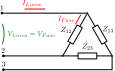
\includegraphics[width=0.6\linewidth]{Imagenes/motorParte2.png}
\caption{Motor asicrónico trifásico de inducción - Conexión triángulo}
\end{figure}

De la placa se obtiene que $V_{Fase} = 230V$, y la $I_{Fase} = 0.42A$. Dado el $cos(\phi) = 0.75$, se obtiene la fase $\phi = 41^{\circ}$. Se calcula entonces las impedancias a usar como modelo:

\[
Z = \frac{|V_{Fase}|}{|I_{Fase}|} \phase{44^{\circ}} = 547.6\Omega \phase{44^{\circ}} = 410 \Omega + j362 \Omega
\]  

De la parte imaginaria se obtiene el valor de la inductancia para el modelo:

\[
2 \cdot \pi \cdot 50Hz \cdot L = 362\Omega
\]

\[
L = 1.15H
\]

\subsubsection{Simulación en el Inverter - Conexión Triángulo}

Para tener una $V_{Linea}$ (que en este caso es igual a la tensión de fase por estar conectado en triángulo) de 230V (RMS) para realizar la simulación, se elije un índice de modulación $m_a$ mayor a 1 (es decir, sobremodulando) para no tener que aumentar tanto la tensión $V_d$ y así conseguir más potencia. Tomando $m_a = 1.4$, se estima la $V_d$ necesaria:

\[
V_{ab} = \frac{1}{2} \cdot m_a \cdot V_d \Longrightarrow V_d = 328V
\]

El valor anterior se ajustó a 350V para obtener la $I_{Fase}$ buscada (dado que como $m_a > 1$, no estamos en la zona lineal, por lo que no corresponde exactamente al valor mínimo necesario). El valor pico esperado para la $I_{Fase}$ sería $I_{Fase} = 0.72A \cdot \sqrt{2} = 1A$.

\begin{figure}[H]
\centering
\includegraphics[width=0.9\linewidth]{Imagenes/motorTriangulo.pdf}
\caption{Tensión de fase y corriente de fase de una rama}
\end{figure}


















\end{document}